\documentclass[aspectratio=169,UTF8,fontset=fandol]{ctexbeamer}

\usetheme{Madrid}
\usecolortheme{default}
\setbeamertemplate{navigation symbols}{}
\setbeamertemplate{caption}[numbered]

\usepackage{booktabs}
\usepackage{graphicx}
\usepackage{tabularx}
\usepackage{array}
\usepackage{amsmath}
\usepackage{tikz}
\usetikzlibrary{arrows.meta,positioning,calc}

\graphicspath{{../../Image/}}

\definecolor{accentblue}{HTML}{4C78A8}
\definecolor{accentorange}{HTML}{F58518}
\definecolor{accentred}{HTML}{E45756}
\setbeamercolor{structure}{fg=accentblue}

\title{基于 TCP 通信的联邦学习系统}
\subtitle{计算机网络大作业 Poster 辅助说明}
\author{小组汇报}
\date{2026年6月}

\hypersetup{
  pdftitle={基于 TCP 通信的联邦学习系统},
}

\newcommand{\fig}[2]{%
  \centering
  \includegraphics[width=#1\linewidth]{#2}%
}

\tikzset{
  flowbox/.style={draw, rounded corners=2pt, align=center, minimum width=2.62cm,
    minimum height=0.78cm, font=\small, fill=blue!9},
  orangebox/.style={draw, rounded corners=2pt, align=center, minimum width=2.62cm,
    minimum height=0.78cm, font=\small, fill=orange!16},
  redbox/.style={draw, rounded corners=2pt, align=center, minimum width=2.62cm,
    minimum height=0.78cm, font=\small, fill=red!10},
  arrow/.style={-{Latex[length=2mm]}, line width=0.7pt, draw=gray!70}
}

\begin{document}

\begin{frame}
  \titlepage
\end{frame}

\section{目标与架构}

\begin{frame}{项目目标：用纯 TCP 跑通联邦学习闭环}
  \begin{columns}[c,onlytextwidth]
    \begin{column}{0.55\linewidth}
      \begin{itemize}
        \item 基础任务：1 个 Server + 3 个 Client 的同步式联邦学习。
        \item 网络要求：只使用 Python 原生 \texttt{socket}，不使用 HTTP/RPC 传模型。
        \item 关键难点：模型权重是大 payload，必须解决 TCP 字节流粘包。
        \item 扩展实现：Ring 去中心化、SplitFed、弱网与掉队者、实时监控。
      \end{itemize}
    \end{column}
    \begin{column}{0.41\linewidth}
      \begin{block}{最终结果}
        \centering
        Centralized：99.00\%\\[0.12cm]
        Ring：99.01\%\\[0.12cm]
        SplitFed：99.04\%
      \end{block}
      \begin{alertblock}{展示重点}
        网络协议和弱网容错是本项目的核心，不只是模型训练。
      \end{alertblock}
    \end{column}
  \end{columns}
\end{frame}

\begin{frame}{集中式联邦学习架构}
  \begin{columns}[c,onlytextwidth]
    \begin{column}{0.52\linewidth}
      \fig{0.95}{centralized.png}
    \end{column}
    \begin{column}{0.44\linewidth}
      \begin{itemize}
        \item Server 保存全局 CNN 和测试集。
        \item Client 只读取自己的本地数据文件。
        \item 每轮流程：广播权重、Client 本地训练、上传更新、FedAvg 聚合。
        \item 达到目标准确率后广播 shutdown。
      \end{itemize}
    \end{column}
  \end{columns}
\end{frame}

\section{TCP 协议}

\begin{frame}{自定义 TCP 封包解决粘包问题}
  \centering
  \begin{tikzpicture}
    \node[flowbox, minimum width=2.8cm, fill=blue!12] (len) {Length Header\\8 字节};
    \node[orangebox, right=0.18cm of len, minimum width=2.6cm] (magic) {Magic Number\\\texttt{SF26}};
    \node[redbox, right=0.18cm of magic, minimum width=4.2cm] (payload) {Payload\\pickle + 可选 gzip};
  \end{tikzpicture}

  \vspace{0.5cm}
  \begin{columns}[T,onlytextwidth]
    \begin{column}{0.48\linewidth}
      \begin{block}{发送端}
        \small
        \begin{itemize}
          \item \texttt{pickle.dumps(message)}
          \item \texttt{struct.pack(">Q", length)}
          \item \texttt{sendall(header + magic + payload)}
        \end{itemize}
      \end{block}
    \end{column}
    \begin{column}{0.48\linewidth}
      \begin{block}{接收端}
        \small
        \begin{itemize}
          \item 先精确读 8 字节长度。
          \item 再精确读 4 字节魔数。
          \item 最后循环接收，直到读满 L 字节。
        \end{itemize}
      \end{block}
    \end{column}
  \end{columns}
\end{frame}

\begin{frame}{基础训练流程}
  \centering
  \begin{tikzpicture}[node distance=0.48cm]
    \node[flowbox] (reg) {Client 注册};
    \node[flowbox, right=of reg] (broadcast) {Server 广播\\全局权重};
    \node[flowbox, right=of broadcast] (train) {Client 本地\\训练 1 epoch};
    \node[flowbox, right=of train] (upload) {上传模型\\更新};
    \node[flowbox, right=of upload] (avg) {FedAvg\\加权聚合};
    \foreach \a/\b in {reg/broadcast,broadcast/train,train/upload,upload/avg}
      \draw[arrow] (\a) -- (\b);
  \end{tikzpicture}

  \vspace{0.65cm}
  \begin{itemize}
    \item 每个 Client 的上传消息包含权重、样本数、训练/验证/测试指标。
    \item Server 按样本数加权平均：$w=\sum_i \frac{n_i}{\sum_j n_j} w_i$。
    \item 每轮结束后 Server 在全局测试集上评估并记录网络传输统计。
  \end{itemize}
\end{frame}

\section{弱网与扩展}

\begin{frame}{弱网处理：延迟发生在 Client，决策发生在 Server}
  \begin{columns}[T,onlytextwidth]
    \begin{column}{0.48\linewidth}
      \begin{block}{Client 侧模拟}
        \small
        \begin{itemize}
          \item 配置：\texttt{client\_2.delay = 5.0}
          \item 本地训练完成后，发送更新前 sleep。
          \item 可配置 \texttt{drop\_rate} 直接跳过某轮上传。
          \item 上报 \texttt{straggler\_delay} 监控事件。
        \end{itemize}
      \end{block}
    \end{column}
    \begin{column}{0.48\linewidth}
      \begin{alertblock}{Server 侧容错}
        \small
        \begin{itemize}
          \item \texttt{server\_timeout} 控制最多等待时间。
          \item 超时后未返回节点记为 \texttt{straggler\_dropped}。
          \item 若收到数 $\ge$ \texttt{min\_clients}，继续聚合。
          \item 否则中止本次训练。
        \end{itemize}
      \end{alertblock}
    \end{column}
  \end{columns}
\end{frame}

\begin{frame}{扩展一：Ring 去中心化拓扑}
  \begin{columns}[c,onlytextwidth]
    \begin{column}{0.52\linewidth}
      \fig{0.92}{ring.png}
    \end{column}
    \begin{column}{0.44\linewidth}
      \begin{itemize}
        \item 废弃中心 Server，三个节点组成环。
        \item Node 1 训练后发给 Node 2，Node 2 再发给 Node 3。
        \item 模型绕环返回 Node 1 后进行全局测试。
        \item 优点是无中心节点；代价是节点之间串行依赖更强。
      \end{itemize}
    \end{column}
  \end{columns}
\end{frame}

\begin{frame}{扩展二：SplitFed 分割联邦}
  \begin{columns}[c,onlytextwidth]
    \begin{column}{0.52\linewidth}
      \fig{0.92}{splitfed.png}
    \end{column}
    \begin{column}{0.44\linewidth}
      \begin{itemize}
        \item Client 保存 CNN 前半段，Server 保存后半段。
        \item Client 每个 batch 发送激活值和标签。
        \item Server 计算 loss 与梯度，再把激活梯度传回 Client。
        \item 收敛轮次少，但 batch 级通信导致通信量最大。
      \end{itemize}
    \end{column}
  \end{columns}
\end{frame}

\section{实验结果}

\begin{frame}{三种模式结果对比}
  \centering
  \small
  \begin{tabular}{lrrrr}
    \toprule
    模式 & 完成轮次 & 测试准确率 & 运行时长 & 网络收发量 \\
    \midrule
    Centralized & 6 / 10 & 0.9900 & 192.5s & 58.0 MB / 58.0 MB \\
    Ring & 9 / 10 & 0.9901 & 214.1s & 43.5 MB / 43.5 MB \\
    SplitFed & 4 / 10 & 0.9904 & 334.2s & 9.0 GB / 9.0 GB \\
    \bottomrule
  \end{tabular}

  \vspace{0.55cm}
  \begin{alertblock}{结论}
    \small Centralized 最符合基础要求且总耗时最短；Ring 证明去中心化可行；SplitFed 准确率略高但通信开销最大。
  \end{alertblock}
\end{frame}

\begin{frame}{监控面板与训练曲线}
  \begin{columns}[c,onlytextwidth]
    \begin{column}{0.49\linewidth}
      \centering
      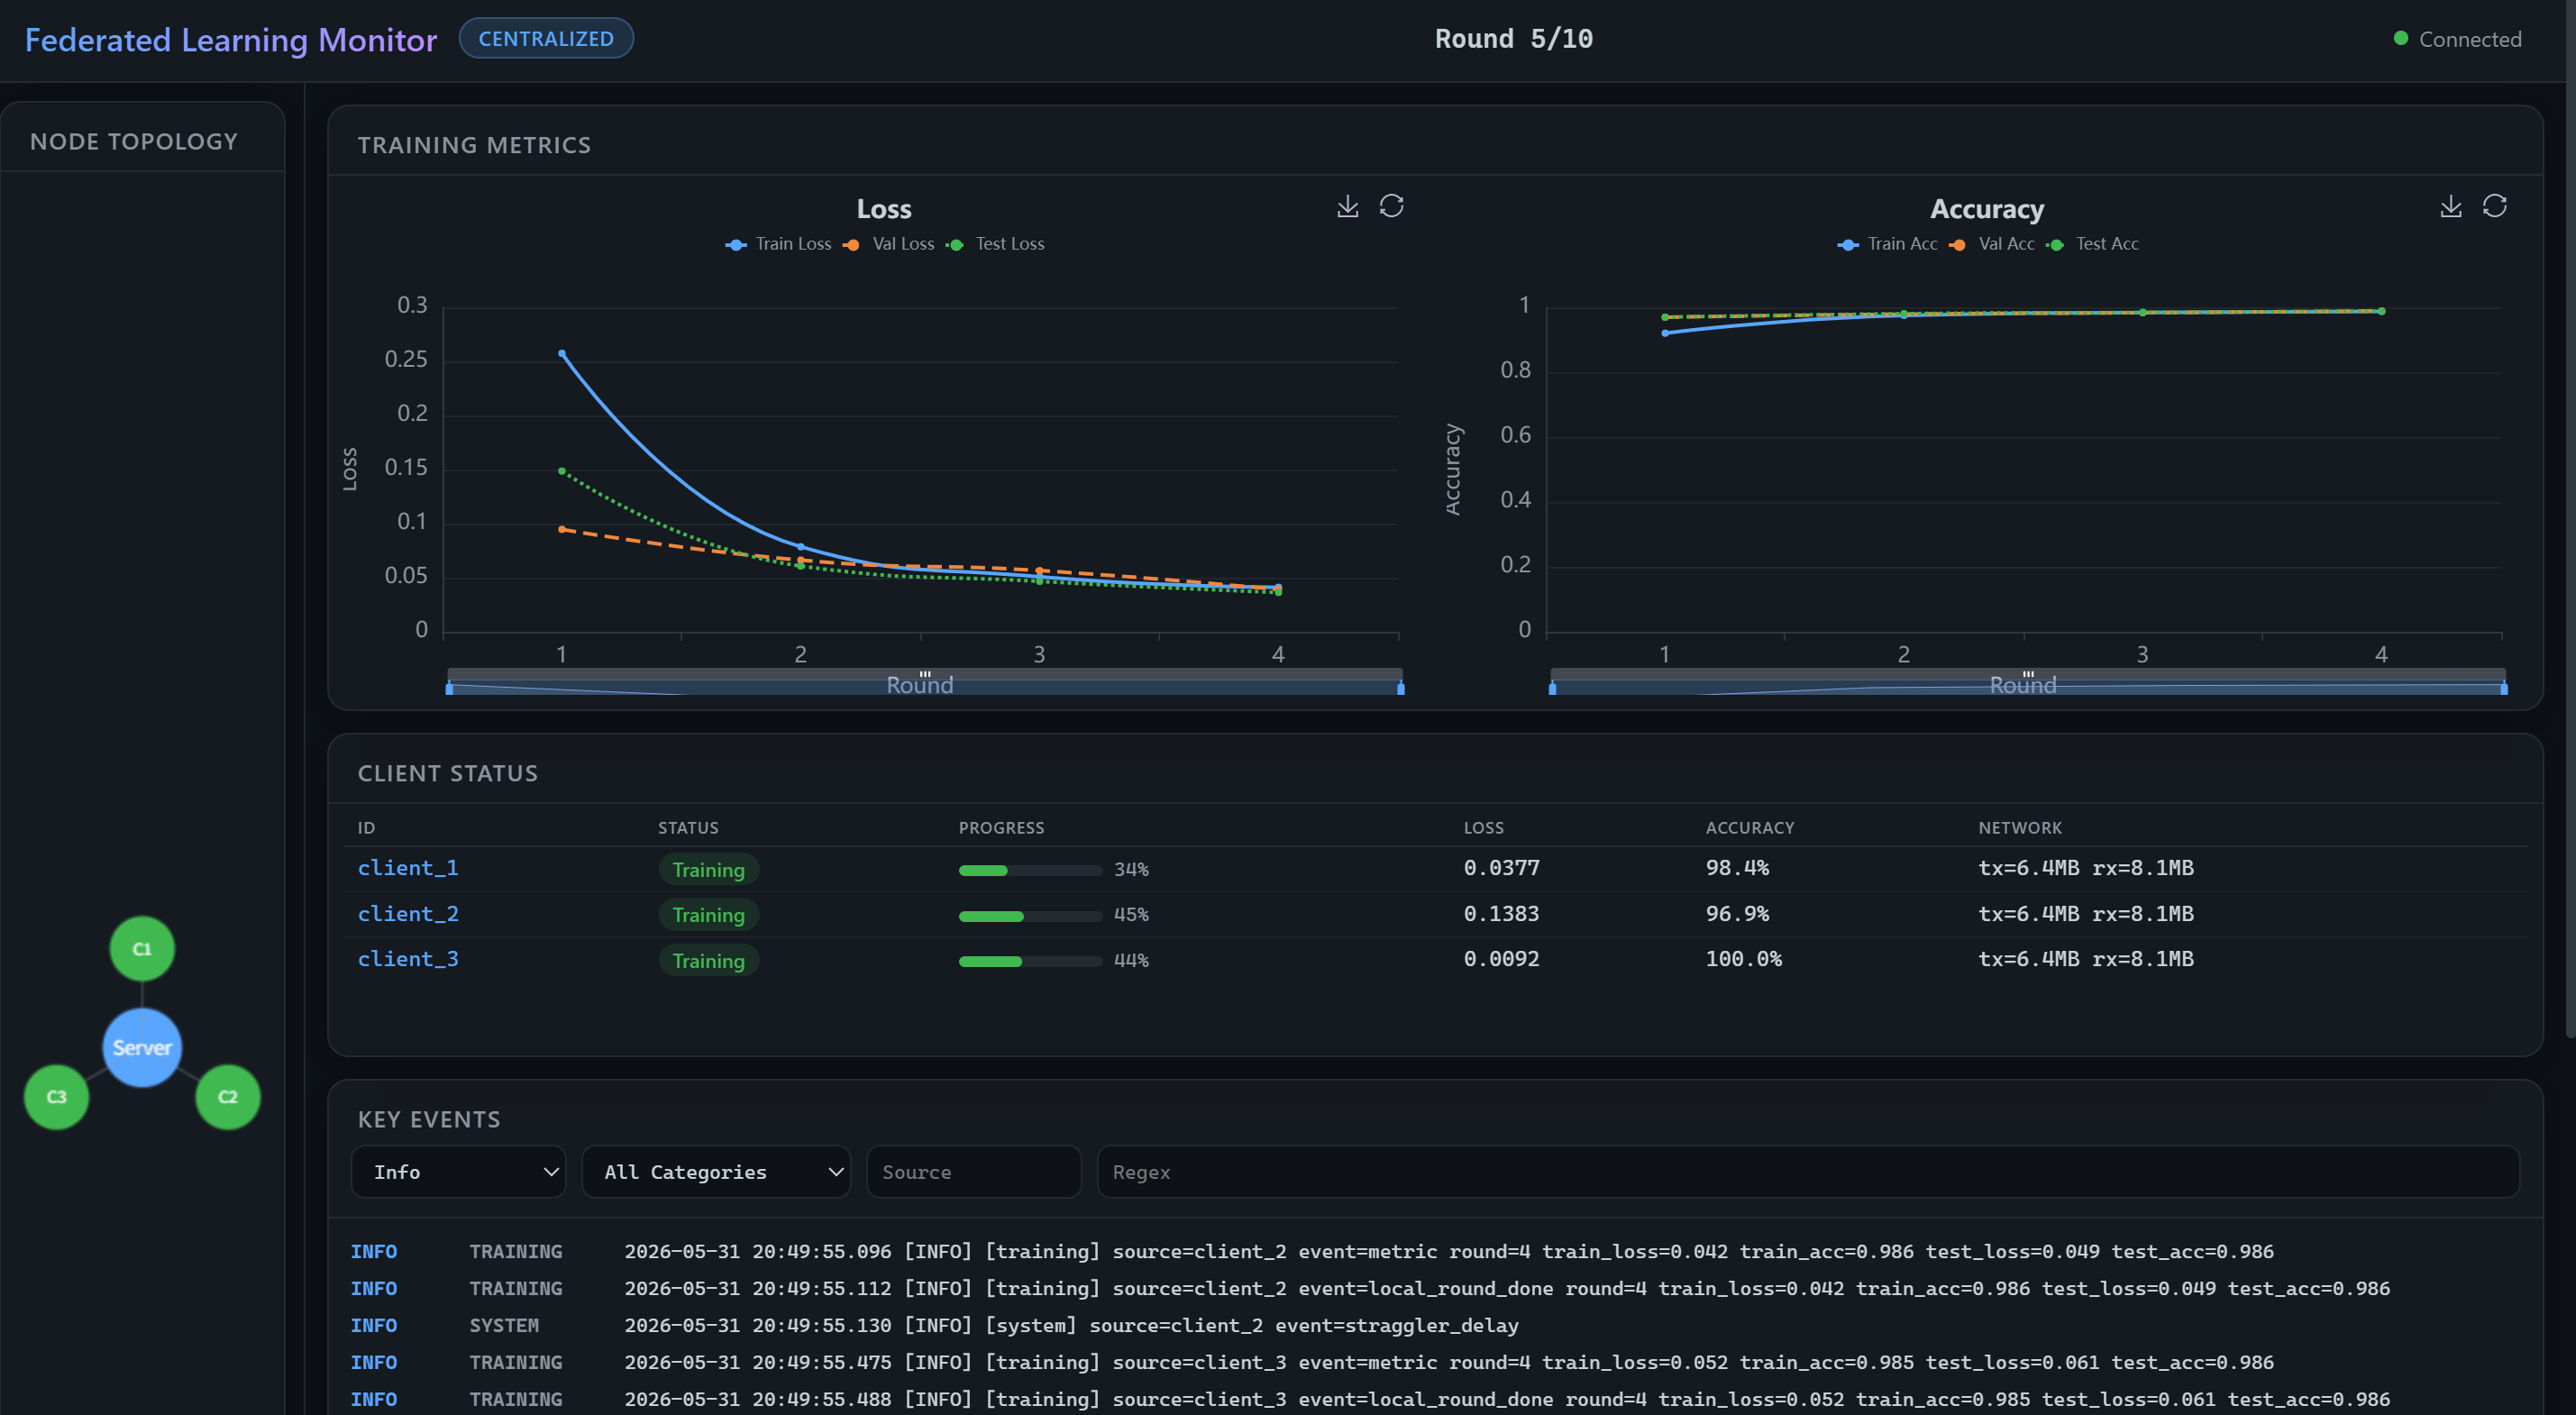
\includegraphics[width=0.96\linewidth,height=0.66\textheight,keepaspectratio]{centralized-overall.png}
    \end{column}
    \begin{column}{0.49\linewidth}
      \centering
      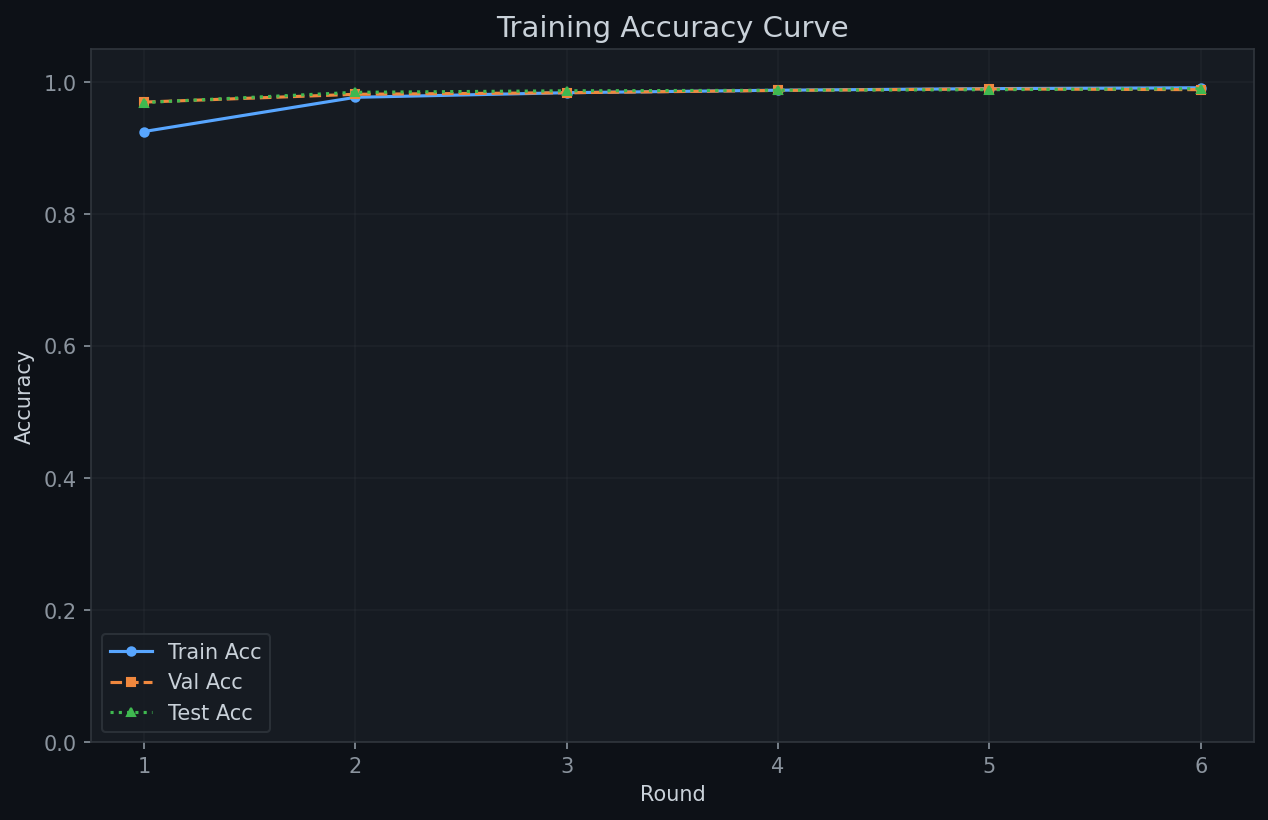
\includegraphics[width=0.96\linewidth,height=0.30\textheight,keepaspectratio]{centralized-accuracy-curve.png}
      \vspace{0.04cm}
      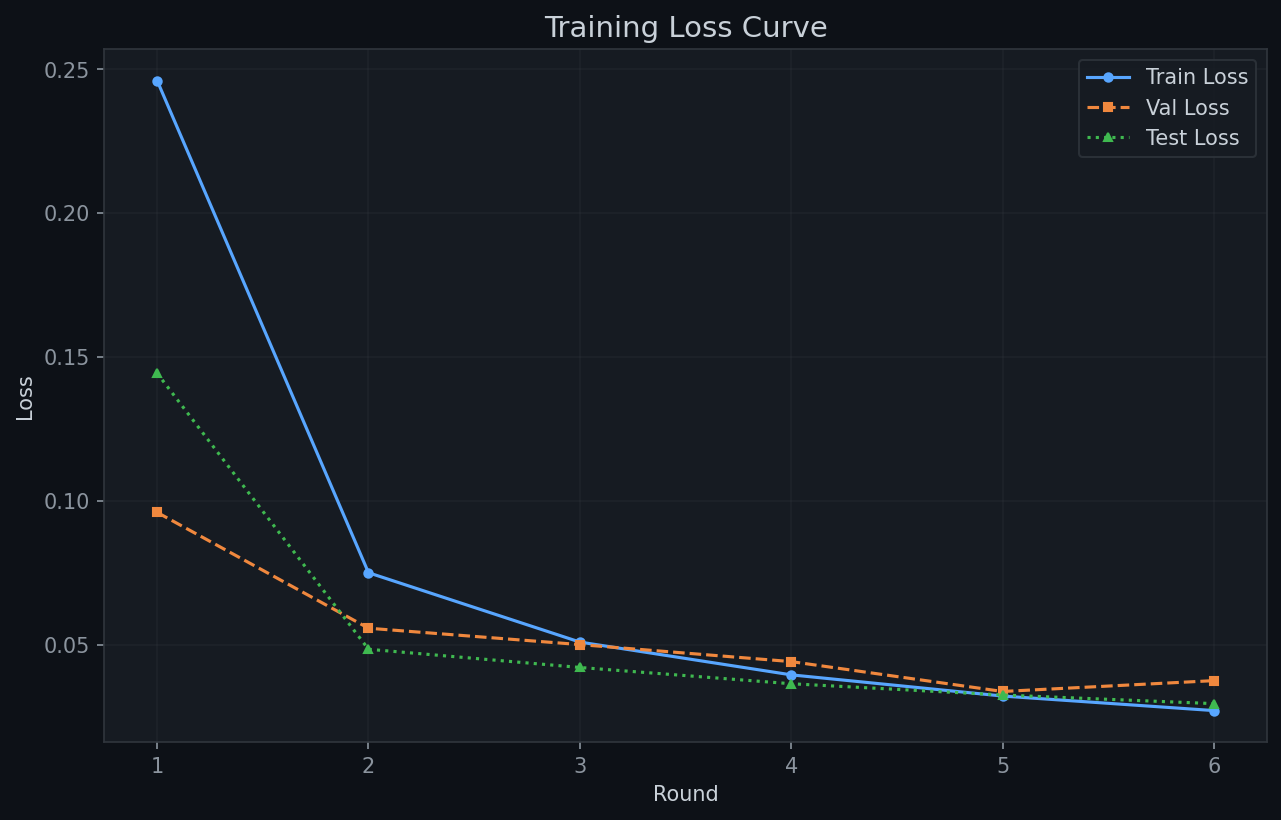
\includegraphics[width=0.96\linewidth,height=0.30\textheight,keepaspectratio]{centralized-loss-curve.png}
    \end{column}
  \end{columns}
\end{frame}

\end{document}
